%include tikz if not already done
%\@ifpackageloaded{tikz}{}{\usepackage{tikz}} %T->nothing F->usepackage
%\usepackage{tikz}

%define functions for squares
\newcommand{\square}[3]{%kwargs x0, y0, width/2
  \draw (#1-#3, #2-#3) -- (#1-#3, #2+#3)
  -- (#1+#3, #2+#3) -- (#1+#3, #2-#3)
  -- (#1-#3, #2-#3);
}

\newlength{\halfwidthnuclides}
\newlength{\distancenuclides}
\setlength{\halfwidthnuclides}{5mm}
\setlength{\distancenuclides}{4\halfwidthnuclides}

\usetikzlibrary{patterns}

\begin{figure}
  \centering
  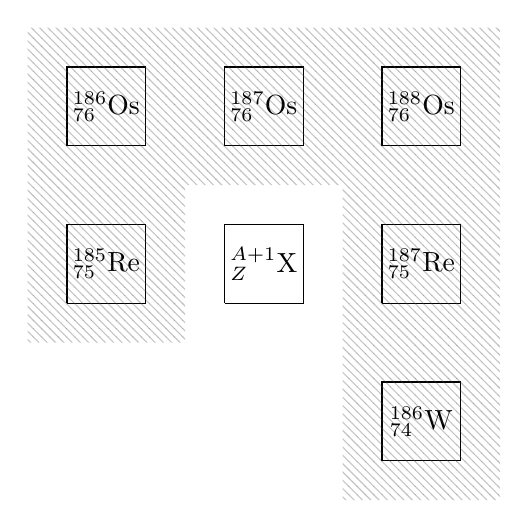
\begin{tikzpicture}
    %test in the middle
    \draw (0,0) node {${}^{A+1}_{Z}$X};
    \square{0}{0}{\halfwidthnuclides}
    %Os-row on top of test
    \draw (-\distancenuclides,\distancenuclides) node {${}^{186}_{76}$Os};
    \square{-\distancenuclides}{\distancenuclides}{\halfwidthnuclides}
    \draw (0,\distancenuclides) node {${}^{187}_{76}$Os};
    \square{0}{\distancenuclides}{\halfwidthnuclides}
    \draw (\distancenuclides,\distancenuclides) node {${}^{188}_{76}$Os};
    \square{\distancenuclides}{\distancenuclides}{\halfwidthnuclides}
    %stable Re-isotopes
    \draw (-\distancenuclides,0) node {${}^{185}_{75}$Re};
    \square{-\distancenuclides}{0}{\halfwidthnuclides}
    \draw (\distancenuclides,0) node {${}^{187}_{75}$Re};
    \square{\distancenuclides}{0}{\halfwidthnuclides}
    %W island of stability
    \draw (\distancenuclides,-\distancenuclides) node {${}^{186}_{74}$W};
    \square{\distancenuclides}{-\distancenuclides}{\halfwidthnuclides}
    %shaded region of stability
    \fill[color=lightgray,opacity=0.3, pattern=north west lines, pattern color=darkgray]
    (-0.5\distancenuclides,-0.5\distancenuclides)
    rectangle (-1.5\distancenuclides,1.5\distancenuclides)
    rectangle (1.5\distancenuclides,0.5\distancenuclides)
    rectangle (0.5\distancenuclides,-1.5\distancenuclides);
  \end{tikzpicture}
\end{figure}
